\documentclass[10pt]{article}
\usepackage[usenames]{color} %used for font color
\usepackage{amssymb} %maths
\usepackage{amsmath} %maths
\usepackage{graphicx}
\usepackage[utf8]{inputenc} %useful to type directly diacritic characters
\title{Classifying Handwritten Mathematical Symbols and Analysis of Adam Optimizer}
\author{Yavuz Bakman}

\begin{document}
\maketitle
\section{Introduction}
\hspace{10mm}
Classifiying handwritten numbers is one of the oldest problem in machine learning. Especially, MNIST dataset is such a popular that most of the introduction to classification lectures start with that example. However, classifiying numbers is not enough for the converting mathematical expression into  for instance LATEX format. To do that, we also need convert mathematical symbols such as $ !, \times , - ,+ $ into their ground truth.

\section{Problem}
\hspace{10mm}
In the project, we want to solve the first and crucial step of the converting handwritten mathematical expression into LATEX format which is classifiying handwritten mathematical symbols and numbers. We apply various machine learning model with different  hyperparameters. Also, we explained the main idea of the Adam optimizer. It only explains the theoritical results of the main Adam paper and does not provide any new theoritical results.

\section{Dataset}
\hspace{10mm}
We used the Kaggle dataset \cite{dataset} which consists of 100 000 handwritten mathematical symbol images. The images are grayscale and 45x45 jpg format. There are 82 different symbols including all math operators, set operators, basic pre-defined math functions like: log, lim, cos, sin, tan, math symbols like: $\int, \sum, \sqrt,  \delta$ and more. Original source, that was parsed, extracted and modified is CROHME     \cite{dataset2} dataset.

\section{Methods}
We implemented 4 different methods with various hyperparameters. The best hyperparameter set is selected by the 5-fold validation. Every algorithm will be explained in the corresponding subsections.
\subsection{Softmax Regression}
The first algorithm we apply is softmax regression. It is the linear model for the multiclass classification model. We flatten the image matrix into vector and multiply each pixel with random weights. Then we sum the result of the multiplication after that we add bias term. Now, all we have to do is minimize the cost function which Cross Entropy Loss. There are 82 classes and minibatch size = 50 so:
\begin{align}
-\sum_{i=1}^{50} \sum_{l=1}^{82} 1_{y^(i) = l} \frac  {e^{\theta_l^Tx^{(i)}}}{\sum_{j=1}^{82} e^{\theta_j^Tx^{(i)}}}
\label{equation2}
\end{align}
We use pytorch for the implementation.
\subsection{Support Vector Machines (SVM)}
In support vector machines, the algorithm try to seperates classes by best margin. Here is the equation that SVM wants optimize:
$$
min_{\gamma,w,b} \frac{1}{2}|| w||^2 + C \sum^n_{i=1} \xi_i 
$$
s.t
$$
y^{i}(w^Tx^{i} + b) \geq 1 -  \xi_i, i = 1,...,n
$$
$$
\xi_i   \geq 0, i = 1,...,n
$$
\begin{figure}[h]
\centering
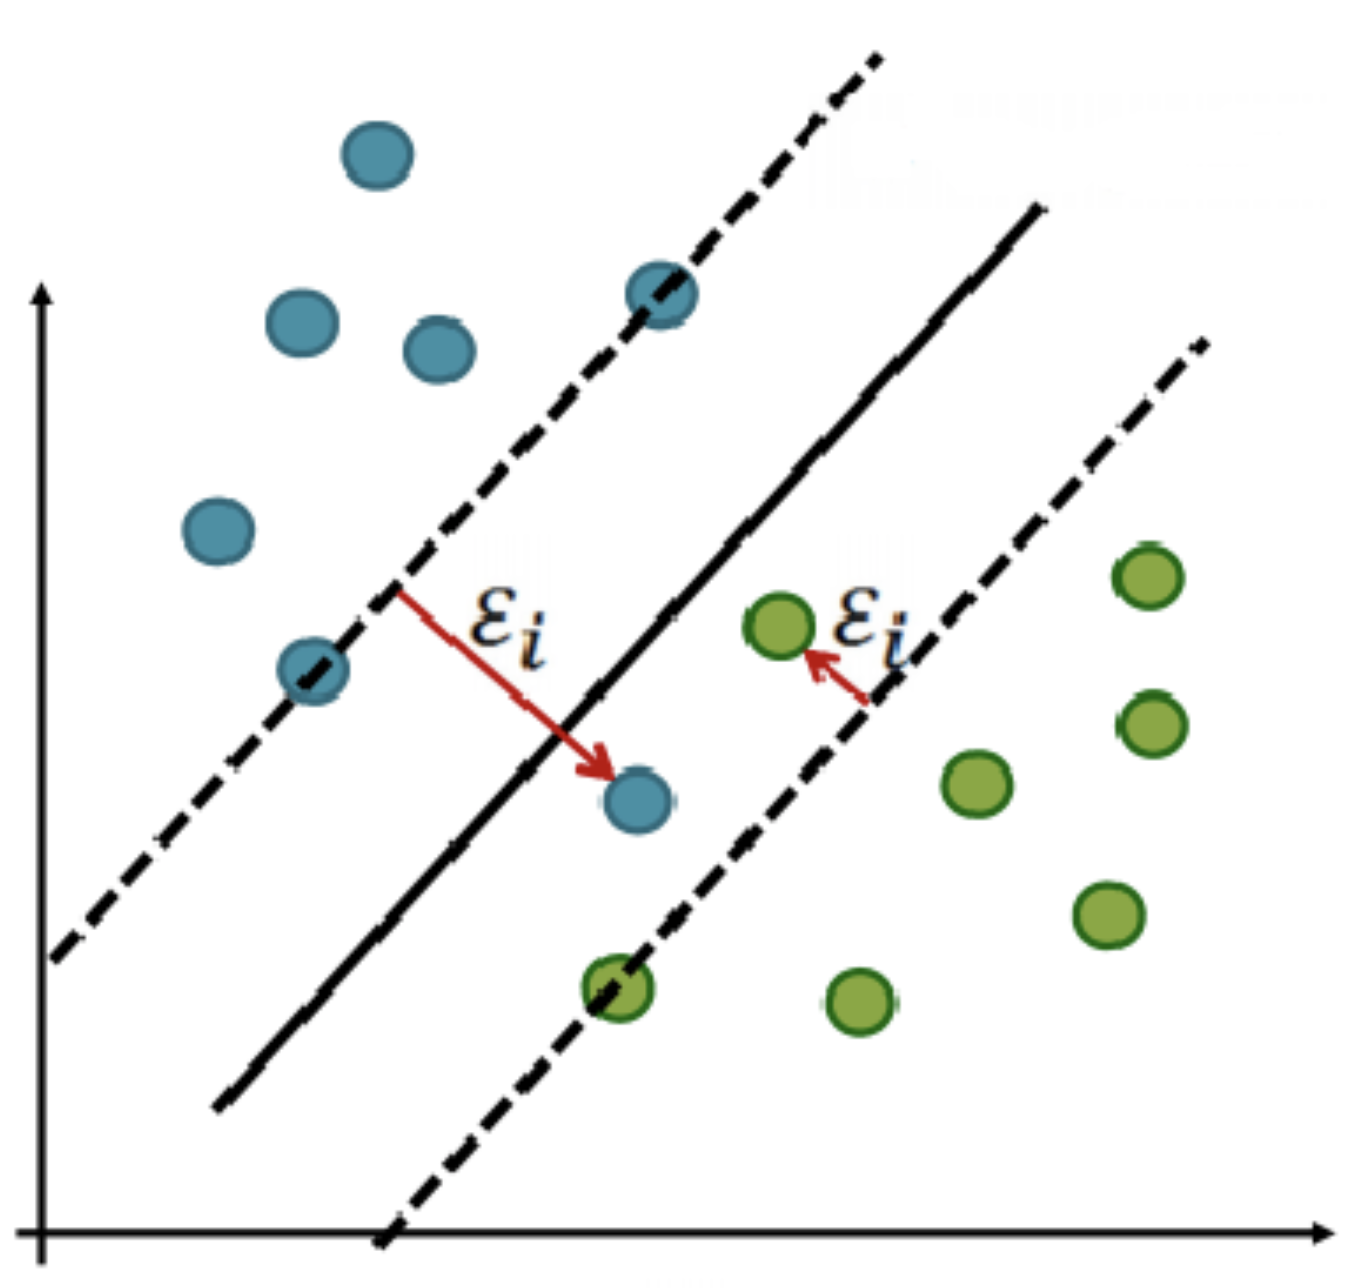
\includegraphics[scale=0.15]{SVM}
\caption{SVM Seperator}
\end{figure}
There are 82 classes. We use one vs rest classification technique. Whole implementation is done by the sckit-learn \cite{sckit}.
\subsection{Multilayer Perceptron (MLP)}
We apply multilayer perceptron model. We use Relu as activation function. Cross Entropy cost function is used. Here is the model:
\begin{figure}[h]
\centering
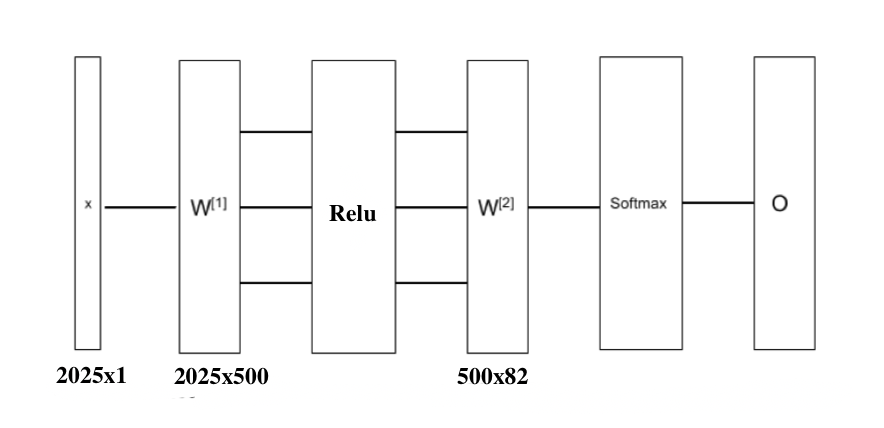
\includegraphics[scale=0.5]{MLP}
\caption{MLP model}
\end{figure}
We implemented the model in pytorch \cite{pytorch}.
\subsection{Convolutional Neural Network (CNN)}
The most modern tecnique we used is convolutional neural networks. In that model, convolutional layers extract feature from the image by considering neighbour pixels. Also, maxpool layers are used to decrease dimension and number of features that makes model easily trainable. Also, it makes rotational/position invariance feature extraction. We use Cross entropy loss function. We try to use Adam and SGD optimizer . The mathematics behind the Adam optimizer will be explained in section 5. The whole implementation is done by pytorch \cite{pytorch} framework. Here is the model:
\begin{figure}[h]
\centering
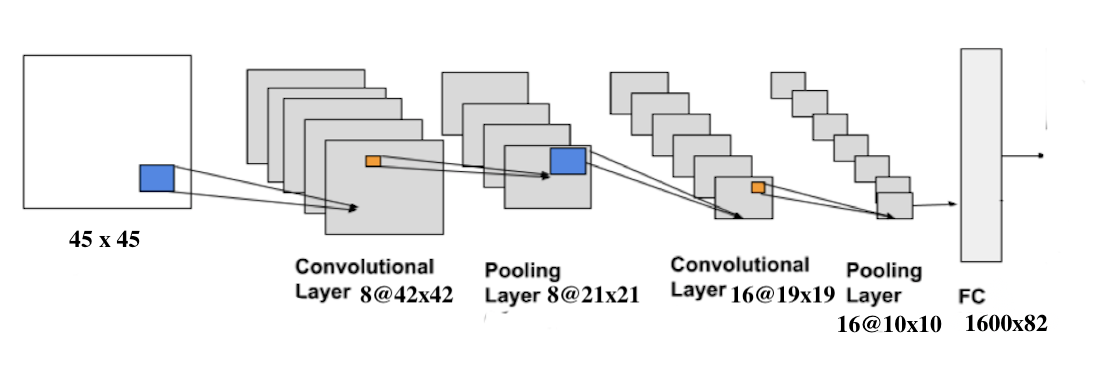
\includegraphics[scale=0.5]{CNN}
\caption{CNN model}
\end{figure} 
\section{Mathematics Behind the Algorithm}
\subsection{Adam Optimizer}
Adam suggests an efficient stochastic optimization method that only needs first order gradient. It is computationally fast and convergence of the algorithm is proven. We show the algorithm and explain the main idea behind the algoritm and also we provide a theoritical analysis of Adam's convergence in online convex programming. Whole proof and the algorithm comes from the original Adam paper \cite{Adam}.
\subsubsection{The Algorithm}
\noindent\rule{12.5cm}{0.4pt}
\textbf{Algorithm:} Adam proposed algorithm for stochastic optimization. $g_t2$ indicates the elementwise square $g_t \odot g_t.$ Good default settings for the tested machine learning problems are $\alpha = 0.001, \beta_1 = 0.9, \beta_2 = 0.999$ and $\epsilon = 10^{-8}$. All operations on vectors are element-wise.\newline
\noindent\rule{12.5cm}{0.4pt}
\textbf{Require:} $\alpha$: Stepsize\newline
\textbf{Require:} $\beta_1 , \beta_2 \in [0, 1)$: Exponential decay rates for the moment estimates \newline
\textbf{Require:} $f(\theta)$: Stochastic objective function with parameters $\theta$\newline
\textbf{Require:}  $\theta_0$: Initial parameter vector\newline
 $m_0 \leftarrow 0$ (Initialize 1st moment vector) \newline
 $v_0 \leftarrow 0$ (Initialize 2nd moment vector) \newline
 $t \leftarrow 0$ (Initialize timestep)\newline
while $\theta_t$ not converged do \newline
$t \leftarrow t+1$ \newline
$g_t   \leftarrow\nabla_{\theta}f_t(\theta_{t-1}) $ (Get gradients w.r.t. stochastic objective at timestep t) \newline
$m_t \leftarrow \beta_1  m_{t-1} + (1 - \beta_1)g_t $ (Update biased first moment estimate) \newline
$v_t \leftarrow \beta_2  v_{t-1} + (1 - \beta_2)  g_t2$ (Update biased second raw moment estimate)  \newline
$\hat m_t \leftarrow m_t /(1-\beta_{1}^t)$(Compute bias-corrected first moment estimate) \newline
$ \hat v_t  \leftarrow v_t /(1 - \beta_2^t )$ (Compute bias-corrected second raw moment estimate) \newline
$ \theta_t \leftarrow \theta_{t-1} - \alpha   \hat m_t /(\sqrt{\hat v_t} + \epsilon)$ (Update parameters) \newline
end while \newline
return $\theta_t$ (Resulting parameters) \newline
\noindent\rule{12.5cm}{0.4pt}
Here is the pseudo-code for the algorithm. $f(\theta)$ is the objective function differantiable with respect to $\theta$. Our main goal is to minimize $E(f(\theta))$. $\nabla_{\theta}f_t(\theta_{t})$ denotes for the gradient which is partial derivatives of objective function evaluated at timestep $t$. $m_t$ and $v_t$ correspond first moment (the mean) and second raw moment (the uncentered variance) of the gradient respectively. These are updated with each iteration. After the rescaling of the gradient, the update happens with learning rate parameter.
\subsubsection{The Convergence Analysis of Adam}
We analyze the converge of the algorithm in online learning framework.We have unknown sequence of convex cost functions $f_1(\theta), f_2(\theta),...,f_T(\theta)$. We analyse the algorithm by regret. Here is the definition of regret:
\begin{align}
R(T) = \sum_{t=1}^{T}[f_t(\theta_t)	- f_t(\theta^*)]
\label{regret}
\end{align}
where $\theta^* = argmin_{\theta} \sum_{t=1}^{T} f_t(\theta_t)$. We show that Adam has $O(\sqrt{T} )$ regret bound.For simplicity, we use some definitions: $g_t = \nabla f_t(\theta_t)$, $g_{t,i}$ as the ith element. We define $g_{1:t,i} = [g_{1,i},g_{2,i}..., g_{t,i} ]$ and also $\gamma = \beta_1^2/\sqrt{\beta_2}$. The following theorem holds when the learning is decaying at a rate of $t{-1/2}$ and first moment running average coefficient $\beta_{1,t}$ decay exponentially with $\lambda$, that is typically close to 1.\newline
\textbf{Theorem:} Assume that the function $f_t$ has bounded gradients, $||\nabla f_t(\theta)||_2 \leq G ,  f_t(\theta)||_{\infty} \leq G_{\infty}$ for all $\theta \in R^d$ and distance between any $\theta_t$ generated by Adam is bounded $||\theta_n - \theta_m||_2 \leq D,  ||\theta_n - \theta_m||_\infty \leq D_\infty$ for any $m,n \in {1,...,T}$ and $\beta_1 , \beta_2 \in [0,1)$ satisfy $\gamma < 1 $. Let $\alpha_t = \alpha/\sqrt{t}$ and $\beta_{1,t} = \beta_1\lambda^{t-1}, \lambda \in (0,1)$ Adam achives the following: $$
R(T) \leq \frac{D^2}{2 \alpha (1-\beta_1)} \sum_{i=1}^d \sqrt{T \hat{v}_{T,i}} + \frac{\alpha(1 + \beta_1) G_\infty}{(1-\beta_1) \sqrt{1-\beta_2}(1-\gamma)^2} \sum_{i=1}^d ||g_{1:T,i} ||_2 + \sum_{i=1}^d \frac{D^2_\infty G_\infty \sqrt{1-\beta_2}}{2\alpha(1-\beta_1)(1-\lambda)^2}$$
\textbf{Proof:} We put some lemmas for the main proof but we skip the proof of the lemmas because of the space issues of that paper. You can find the proof of the lemmas in the main paper \cite{Adam}. \newline
\textbf{Lemma 1.:} If a function $f: R^d \rightarrow R$ is convex, then for all $x,y \in R^d$
$$ f(y) \geq f(x) + \nabla f(x)^T(y-x) $$
\textbf{Lemma 2.:} Let $g_t = \nabla f_t(\theta_t)$ and $g_{1:t}$ be defined as above and bounded, $||g_t||_2 \leq G, ||g||_\infty \leq G_\infty$ then,
$$ \sum_{t=1}^T \sqrt{g^2_{t,i}/t} \leq 2G_\infty||g_{1:T,i} ||_2$$
\textbf{Lemma 3.:} Let $\gamma = \beta_1^2/\sqrt{\beta_2}$. For $\beta_1, \beta_2 \in [0,1)$ that satisfy $\beta_1^2/\sqrt{\beta_2} < 1$ and bounded $g_t, ||g_t||_2 \leq G, ||g_t||_\infty \leq G_\infty$ the following inequality holds:
$$  \sum^T_{t=1} \frac{\hat{m}^2_{t,i}}{\sqrt{t\hat{v}_{t,i}}} \leq \frac{2}{1-\gamma} \frac{1}{\sqrt{1-\beta_2}} ||g_{1:T,i}||_2
$$ 
\textbf{Proof of the Theorem.:} By first lemma: 
$$
f_t(\theta_t) - f_t(\theta^*) \leq g_t^T(\theta_t - \theta^*) \leq \sum_{i=1}^d g_{t,i}(\theta_{i,d}-\theta_i^*)
$$
By the update rule from the Algorithm:
\begin{align*}
\theta_{t+1} &= \theta{t} - \alpha_t \hat{m}_t / \sqrt{\hat{v_t}} \\
&= \theta_t - \frac{\alpha_t}{1-\beta_1^t}(\frac{\beta_{1,t}}{\sqrt{\hat{v}_t}} m_{t-1} + \frac{(1-\beta_{1,t})}{\sqrt{\hat{v}_t}})g_t
\end{align*}
We focus on the ith dimension of the parameter vector $\theta \in R^d$. Subtract the scalar $\theta^*$ and square both sides of the above update rule, we have:
$$
(\theta_{t+1} - \theta^*_i)^2 = (\theta_{t} - \theta^*_i)^2 - \frac{2 \alpha_t}{1-\beta^t_1}(\frac{\beta_{1,t}}{\sqrt{\hat{v}_{t,i}}}m_{t-1,i} + (1- \frac{\beta_{1,t}}{\sqrt{\hat{v}_{t,i}}} g_{t,i})(\theta_{t} - \theta^*_i) + \alpha^2_t(\frac{\hat{m}_{t,i}}{\sqrt{\hat{v}_{t,i}}})^2
$$
We can rearrange the equation by Young's inequality, $ab \leq a^2/2 + b^2 / 2$. Also, it can be shown that$ \sqrt{\hat{v}_{t,i}} = \sqrt{\sum^t_{j=1}(1-\beta_2)\beta_2^{t-j}g^2_{j,i}} / \sqrt{1-\beta^t_2} \leq ||g_{1:t,i} ||$ and $ \beta_{1,t} \leq \beta_1$ Then:
\begin{align*}
g_{t,i}(\theta_{t,i} - \theta^*_i) &= \frac{(1-\beta^t_1)\sqrt{\hat{v}_{t,i}}}{2 \alpha_t(1-\beta_{1,t})}((\theta_{t,i} - \theta^*_t)^2 - (\theta_{t+1,i} - \theta^*_i)^2 ) \\
&+ \frac{\beta_{1,t} \hat{v}^{1/4}_{t-1,i}}{(1-\beta_{1,t}) \sqrt{\alpha_{t-1}}}(\theta*_i - \theta_{t,i}) \sqrt{\alpha_{t-1}} \frac{m_{t-1,i}}{\hat{v}^{1/4}_{t-1,i}} + \frac{\alpha_t(1-\beta^t_1)\sqrt{\hat{v}_{t,i}}}{2(1-\beta_{1,t})}( \frac{\hat{m}_{t,i}}{ \sqrt{\hat{v}_{t,i}}})^2 \\
&\leq \frac{1}{2 \alpha_t (1 - \beta_1)} ((\theta_{t,i} - \theta^*_t)^2 - (\theta_{t+1,i} - \theta^*_i)^2 ) \sqrt{\hat{v}_{t,i}} + \frac{\beta_{1,t}}{2\alpha_{t-1}(1 - \beta_{1,t})}(\theta_{t,i} - \theta^*_t)^2 \sqrt{\hat{v}_{t-1,i}} \\
&+ \frac{\beta_1 \alpha_{t-1}}{2(1-\beta_1)} \frac{m^2_{t-1,i}}{\sqrt{\hat{v}_{t-1,i}}} + \frac{\alpha_t \hat{m}^2_{t,i}}{2(1-\beta_1) \sqrt{\hat{v}_{t,i}}}
\end{align*}
We apply lemma 3 to the above inequality and derive the regret bound by summing across all the dimensions for $ i \in 1,..,d$ in the upper bound of $f_t(\theta_t) - f_t(\theta^*)$ adn the sequence of convex functions for $ t \in 1,...T$:
\begin{align*}
R(T) &\leq \sum^d_{i=1} \frac{1}{2\alpha_1(1-\beta_1)}(\theta_{1,i} - \theta^*_i)^2 \sqrt{\hat{v}_{1,i}} + \sum_{i=1}^d \sum_{t=2}^T \frac{1}{2(1-\beta_1)}(\theta_{t,i} - \theta^*_i)^2 (\frac{\sqrt{\hat{v}_{t,i}}}{\alpha_t} - \frac{\sqrt{\hat{v}_{t-1,i}}}{\alpha_{t-1}})\\ 
&+ \frac{\beta_1 \alpha G_\infty}{(1-\beta_1) \sqrt{1-\beta_2} (1-\gamma)^2} \sum_{i=1}^d || g_{1:T,}||_2 + \frac{\alpha G_\infty}{(1-\beta_1) \sqrt{1-\beta_2} (1-\gamma)^2} \sum_{i=1}^d || g_{1:T,}||_2 \\
&+ \sum^d_{i=1} \sum^T_{t=1} \frac{\beta_{1,t}}{2 \alpha_t(1-\beta_{1,t})}(\theta^*_i - \theta_{t,i})^2 \sqrt{\hat{v}_{t,i}}
\end{align*}
From the assumption, $||\theta_t  - \theta^*|| \leq D ||\theta_m  - \theta_n|| \leq D_\infty  $ we have:
\begin{align*}
R(T) &\leq \frac{D^2}{2\alpha(1-\beta_1)} \sum_{i=1}^d \sqrt{T\hat{v}_{T,i}} + \frac{\alpha(1+\beta_1) G_\infty}{(1-\beta_1)\sqrt{1 - \beta_2}(1-\gamma)^2} \sum_{i=1}^d ||g_{1:T,i} ||_2 + \frac{D^2_{\infty}}{2\alpha} \sum_{i=1}^d \sum_{t=1}^t \frac{\beta_{1,t}}{(1-\beta_{1,t})} \sqrt{t \hat{v}_{t,i}} \\
&\leq \frac{D^2}{2\alpha(1-\beta_1)} \sum_{i=1}^d \sqrt{T\hat{v}_{T,i}} + \frac{\alpha(1+\beta_1) G_\infty}{(1-\beta_1)\sqrt{1 - \beta_2}(1-\gamma)^2} \sum_{i=1}^d ||g_{1:T,i} ||_2 \\
&+\frac{D^2_{\infty} G_\infty \sqrt{1-\beta_2}}{2\alpha} \sum_{i=1}^d \sum_{t=1}^t \frac{\beta_{1,t}}{(1-\beta_{1,t})} \sqrt{t}
\end{align*}
For the last term, we apply geometric series upper bound:
\begin{align*}
\sum_{t=1}^t \frac{\beta_{1,t}}{(1-\beta_{1,t})} \sqrt{t} &\leq \sum_{t=1}^t \frac{\lambda^{t-1} \sqrt{t}}{(1-\beta_{1})} \sqrt{t} \\
&\leq \sum_{t=1}^t \frac{\lambda^{t-1} \sqrt{t}}{(1-\beta_{1})} t \\
&\leq \sum_{t=1}^t \frac{1}{(1-\beta_{1}) (1-\lambda)^2}  \\
\end{align*}
Now we reach the following inequation and we are done:
$$
R(T) \leq \frac{D^2}{2 \alpha (1-\beta_1)} \sum_{i=1}^d \sqrt{T \hat{v}_{T,i}} + \frac{\alpha(1 + \beta_1) G_\infty}{(1-\beta_1) \sqrt{1-\beta_2}(1-\gamma)^2} \sum_{i=1}^d ||g_{1:T,i} ||_2 + \sum_{i=1}^d \frac{D^2_\infty G_\infty \sqrt{1-\beta_2}}{2\alpha(1-\beta_1)(1-\lambda)^2}$$

\section{Results}
We share the results of the algorithms in the dataset. 80 percent of the data is used as training and remaining is test. We plot the test accuracy, test loss and training loss vs epoch number. 
\subsection{Graphs}
\begin{figure}[h]
\centering
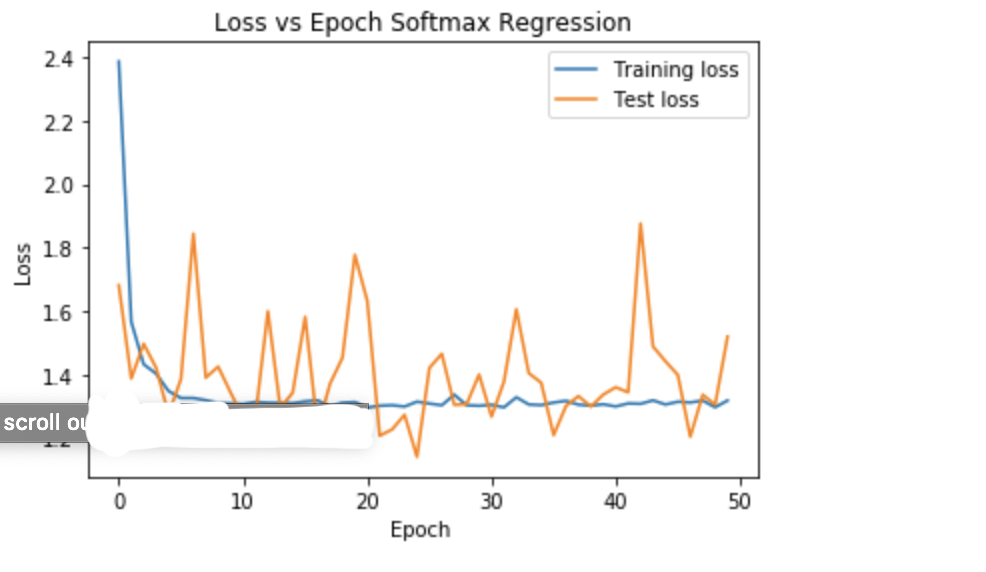
\includegraphics[scale=0.3]{LOSS SOFT}
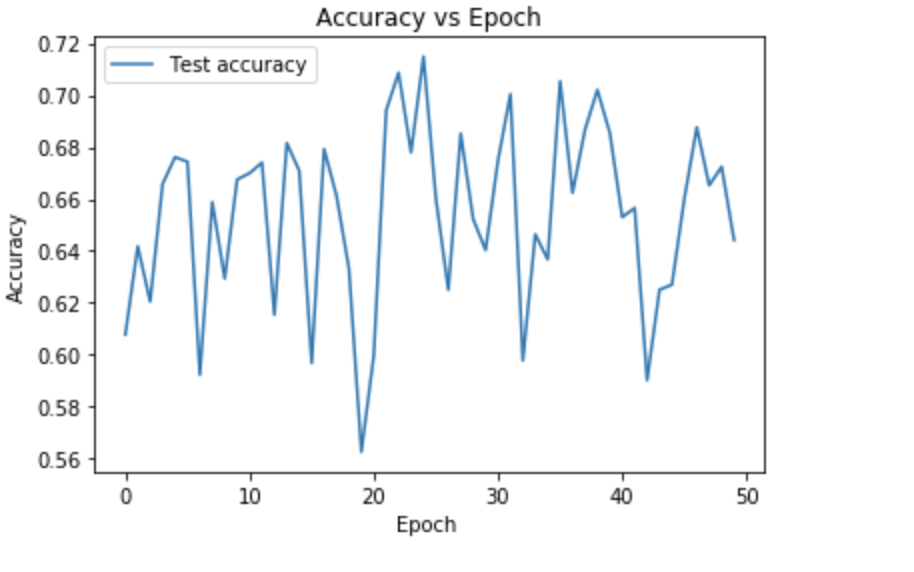
\includegraphics[scale=0.3]{SOFT ACC}
\caption{Softmax Regression Graphs}
\end{figure}
\newpage
\begin{figure}[h]
\centering
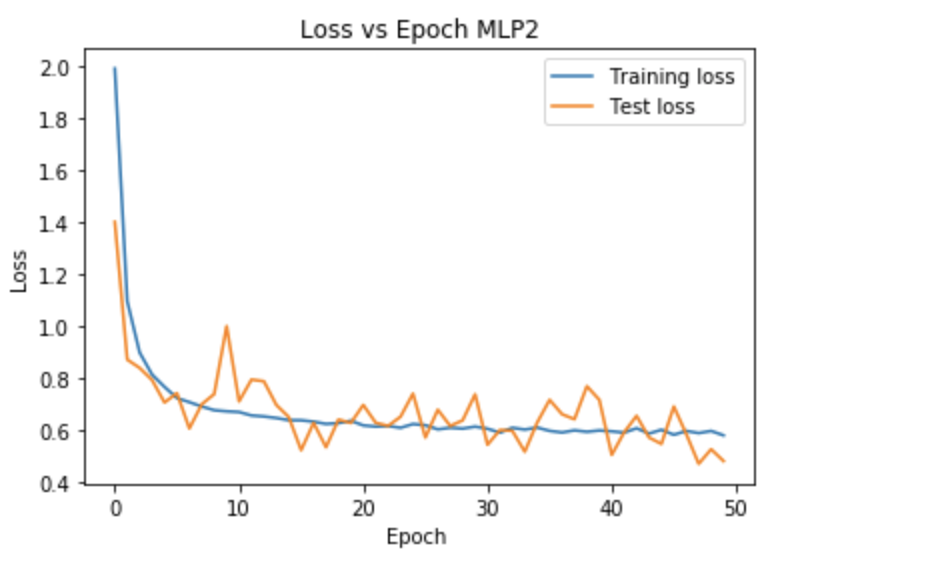
\includegraphics[scale=0.3]{LOSS MLP}
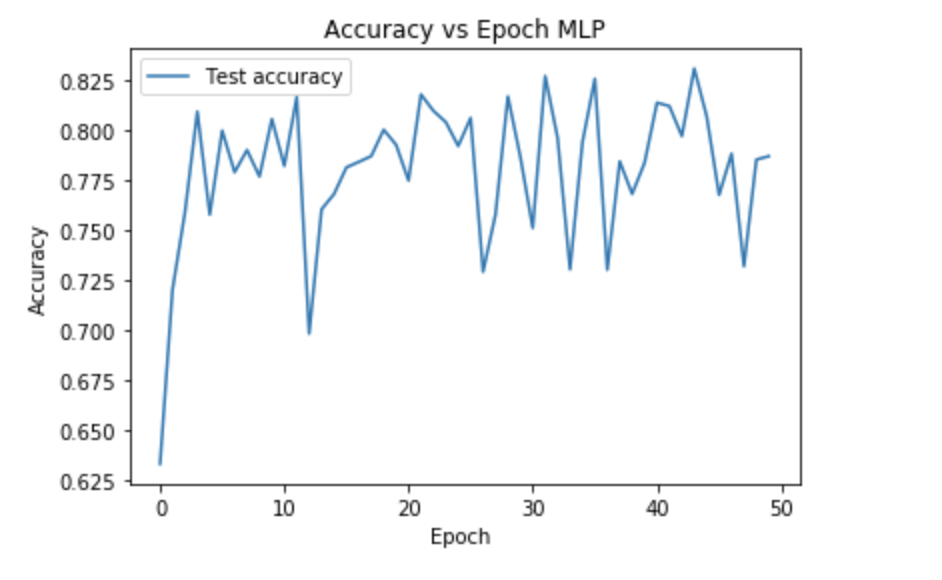
\includegraphics[scale=0.3]{ACC MLP}
\caption{MLP Graphs}
\end{figure}

\begin{figure}[h]
\centering
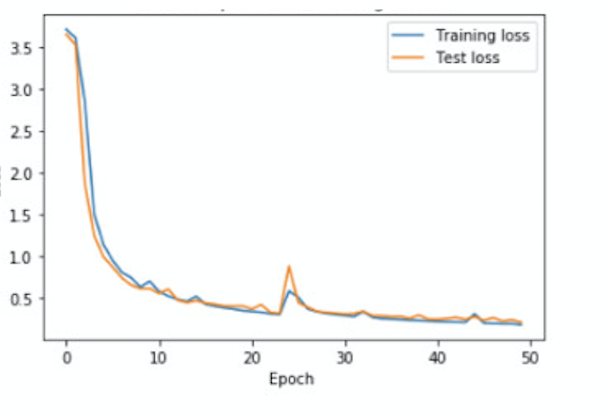
\includegraphics[scale=0.4]{CNN LOSS}
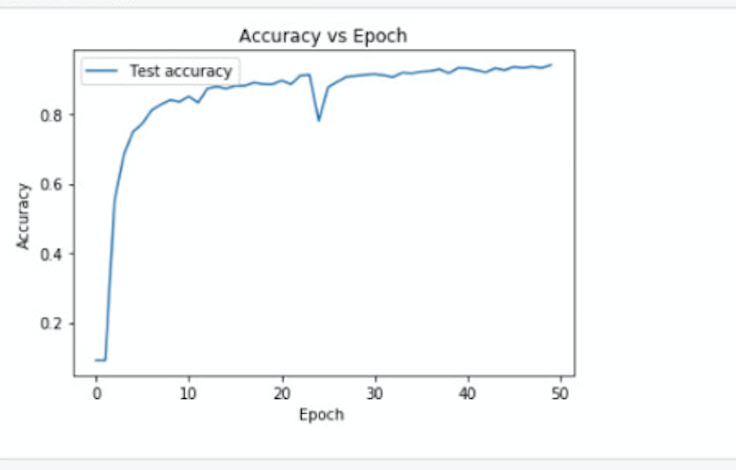
\includegraphics[scale=0.4]{CNN ACC}
\caption{CNN Graphs}
\end{figure}

\begin{table}
\centering
\begin{tabular}{|c|c|}
\hline
Algorithms&Best Accuracy\\
\hline
Softmax Regression&0.655\\
\hline
SVM&0.813\\
\hline
MLP&0.864\\
\hline
CNN&0.943\\
\hline
\end{tabular}
\caption{Accuracy Table}
\end{table}
\subsection{Discussion}
The results of the algorithms are expected. As softmax regression is only a linear model and does not try to make best seperation like it has minimum accuracy. SVM makes the linear seperation better than softmax regression then it has better performance. However, it is still a linear mode. The iideal classification function is propably more complicated than a linear function. MLP has non-linearity by non-linear activation function which is Relu. Therefore, it can classify more than a linear model. However, it stills ignore the neighbour relationship of each pixel. It decreases the performance obviously. CNN handles this problem and it considers other near pixels while extraction feauture from the image. Therefore, it achieves the best performance among all models.
\section{Conclusion}
In the project, we implemented the classification of handwritten symbols and explains the Adam optimizer algorithm. Whole implementation can be found in our github page \cite{github}.





\begin{thebibliography}{2}
\bibitem{dataset} https://www.kaggle.com/xainano/handwrittenmathsymbols
\bibitem{dataset2} http://www.isical.ac.in/~crohme/index.html
\bibitem{pytorch} https://pytorch.org
\bibitem{github} https://github.com/Ybakman/Classifying-Handwritten-Mathematical-Symbols
\bibitem{sckit} https://scikit-learn.org
\bibitem{Adam}Kingma, Diederik P., and Jimmy Ba. "Adam: A method for stochastic optimization." arXiv preprint arXiv:1412.6980 (2014).
\end{thebibliography}
\end{document}